\documentclass[12pt]{article}


\usepackage{amsmath}
\usepackage[margin = 1in]{geometry}
\usepackage{graphicx}
\usepackage{booktabs}
\usepackage{natbib}
\usepackage{multirow}
\usepackage{setspace}
\usepackage[colorlinks=true, citecolor=blue]{hyperref}

\doublespacing


\title{Influences of GDP in the U.S }
\author{Ginamarie Mastrorilli\\
  Department of Statistics\\
  University of Connecticut
}

\begin{document}
\maketitle


\paragraph{Abstract}


\paragraph{Keywords}



\paragraph{Introduction}
%  the introduction sections need to explain the importance of the topic of the paper, provide the background of the research work, and highlight the contributions of the work. At the end of the introduction, a roadmap, or an outline of the paper is useful in helping the readers navigating through the following sections.
%Why does it matter?
%What have been done?
%What is new?

% start with overview 


  What is Gross Domestic Product? Gross Domestic Product is one of the main factors that goes into determining a countries economic growth. 
GDP is the total monetary value of all goods and services that are produced in a country and is a "comprehensive measure of U.S economic activity" \citet[]{bea}.
Gross Domestic Product was originally invented in the 1600's but evolved into governmental use in the 1900's. 
GDP became a national tool to measure a countries economic activity in the 1940's after the Bretton Woods confrence in New Hampshire, US.
At this time, Gross National Product was still a main tool to measure production, but in 1991, the United States swiched to using GDP as its main estimate. 
GDP is calculated by the equation: 

\begin{equation}
C + I + G + NX = GDP
\end{equation}


In this equation, "(C) represents private-consumption expenditures by households and nonprofit organizations, investment (I) refers to business expenditures by businesses and home purchases by households, 
government spending (G) denotes expenditures on goods and services by the government, and net exports (NX) represents a nation’s exports minus its imports." (CITE BRITICANICA)
This equation is one that is learned in any introduction to macroeconomics courses. 
Calculating GDP is something that economists have accomplished and this equation is accepted in the industry. 
What economists are now researching is what factors impact Gross Domestic Product. 
There has been an abdunace of research in this field related to what variables are significant. 
Which factors have been researched are subjective based on those who are conducting the study.



% existing works 
\citet{divya2014study} found that exchange rates and market indexes are important factors that influence an economies GDP. They also found that inflation is highly correlated, but not a significant influencer.  

(cite GDP PARAdox) researches the critism behind GDP's influence in economies. They compare the understanding that even though GDP can influence economically relevant decisions, it does not factor in social welfare. 
Since GDP is a global indicator "The importance of GDP information for firms, investors and citizens/consumers is illustrated by the media – television, radio, newspapers, financial and other magazines, and internet – informing us on a daily basis about the status of our national GDP, both over time and in comparison with other countries." (cite PARADOX)
They also touch on how government agencies and politicians strive to avoid low GDP. When GDP is low, this can lead to negative voter response, and less public expenditures, which are both fatal prospects for those in power (cite PARADOX) 



Szustak found that the relationship between power production and GDP is random. This 



Kalyoncu found that there is "unidirectional causality from per capita GDP to per capita energy consumption for Armenia."(cite dergipark thing). Their research focused on the relationship between energy consumption and economic growth.
The countries they focused their study on, Georgia, Azerbaijan and Armenia from 1995 to 2009, all faced low energy supply. 
% roadmap and contributions

For this paper, we will quantify the relation between influencers of GDP. 






\paragraph{Data}
%Who collected the data (source)? How was the data collected? Sampling frame? Sampling approach? What period or range does the data cover?

The economic data used in this research was collected from Federal Reserve Economic Data(FRED). This is an online database that is maintained by the Research Department at the Federal Reserve Bank of St. Louis. 
The variables collected from the FRED website are Gross Domestic Product (Billions of Dollars, Quarterly, Seasonally Adjusted Annual Rate), Population (Thousands, Quarterly, Not Seasonally Adjusted), Market Yield on U.S. Treasury Securities at 10-Year Constant Maturity, Disposable Personal Income (Billions of Dollars, Quarterly, Seasonally Adjusted Annual), Unemployment Rate (Percent, Quarterly, Seasonally Adjusted), and Business Sector: Labor Productivity (Output per Hour) for All Employed Persons. 


The variable Total Primary Energy Consumption (Quadrillion Btu) used in this research was collected from the U.S. Energy Information Administration website. 
The EIA "collects, analyzes, and disseminates independent and impartial energy information to promote sound policymaking, efficient markets, and public understanding of energy and its interaction with the economy and the environment."(EIA)
My independent variables are Population (POP), Business Sector Labor Productivity (BSLP), 10 Year Treasury Constant Maturity Rate (TCMR), Disposable Personal Income (DPI), Unemployment Rate (UNRATE), and Total Primary Energy Consumption (TPEC). The dependent variable is Gross Domestic Product (GDP).
Observations are taken quarterly from January 1st, 1973 to July 1st, 2022. In this dataframe there are 199 observations from 7 variables with no missing values. 
Summary statistics for the data is as follows






\begin{tabular}{ |p{2cm}||p{2cm}|p{2cm}|p{2cm}|p{2cm}|p{2cm}|p{2cm}|p{2cm}|p{2cm}|}
  \hline
  \multicolumn{9}{|c|}{Summary} \\
  \hline
  Variable & Min. & 1st Quantile & Median & Mean & 3rd Quantile & Max. \\
  \hline
  TPEC & 5.669 & 6.07& 7.609 & 7.462 & 8.082 & 9.965\\
  GDP &  1377 & 4341 & 8363 & 9962 & 14940 & 25248\\
  POP & 211192 & 238482 & 271709 & 273195 & 30886 & 332940\\
  TCMR & .6506 & 3.4607 & 6.1448 & 6.1156 & 8.054 & 14.8384\\
  DPI & 968.7 & 3114.2 & 6037.2 & 7440.5 & 11171.3 & 19586.5\\
  UNRATE & 3.6 & 5.05 & 5.867 & 6.231 & 7.3 & 12.967\\
  BSPL & 45.99 & 56.35 & 67.69 & 75.44 & 98.96\\
  \hline
 \end{tabular}




%Why does the data helps answer the research question?


%What exploratory analyses are done (descriptives, visualication, etc.)?






\paragraph{Methods}

To investigate which factors influence Gross Domestic Product, multiple linear regression will be used. 
Specifically, the variables Population, Business Sector Labor Productivity, 10 Year Treasury Constant Maturity Rate, Disposable Personal Income, Unemployment Rate, and Total Primary Energy Consumption will be used to predict United States Gross Domestic Product.
Multiple linear regrssion is a continuation of simple linear regression. 
For this model, there must be two or more independent predictors that are used to predict one dependent variable. 
The general form of the multiple linear regression model is as follows: 


\begin{equation}
  Y = \beta_0 + \beta_1 X_1 + \beta_2 X_2 + ... + \beta_n X_n + \epsilon
\end{equation}

In this equation, Y is an outcomes that is a continuous measurement. $\beta_0$ is the intercept, $\beta_1 X_1$ is the regression coefficent of the first independent variable. 
$\beta_n X_n$ is the last regression coefficent for the final variable in the model.
$\epsilon$ represents how much variation there is in our estimate for the dependent variable, or otherwise known as model error. 











\paragraph{Application}

When applying multiple linear regression to the data set, all independent variables were included in the intital model.
The model was built using the variables TPEC, POP, TCMR, DPI, UNRATE and BSLP from the traing dataset. 








\begin{figure}[h]
  \centering
  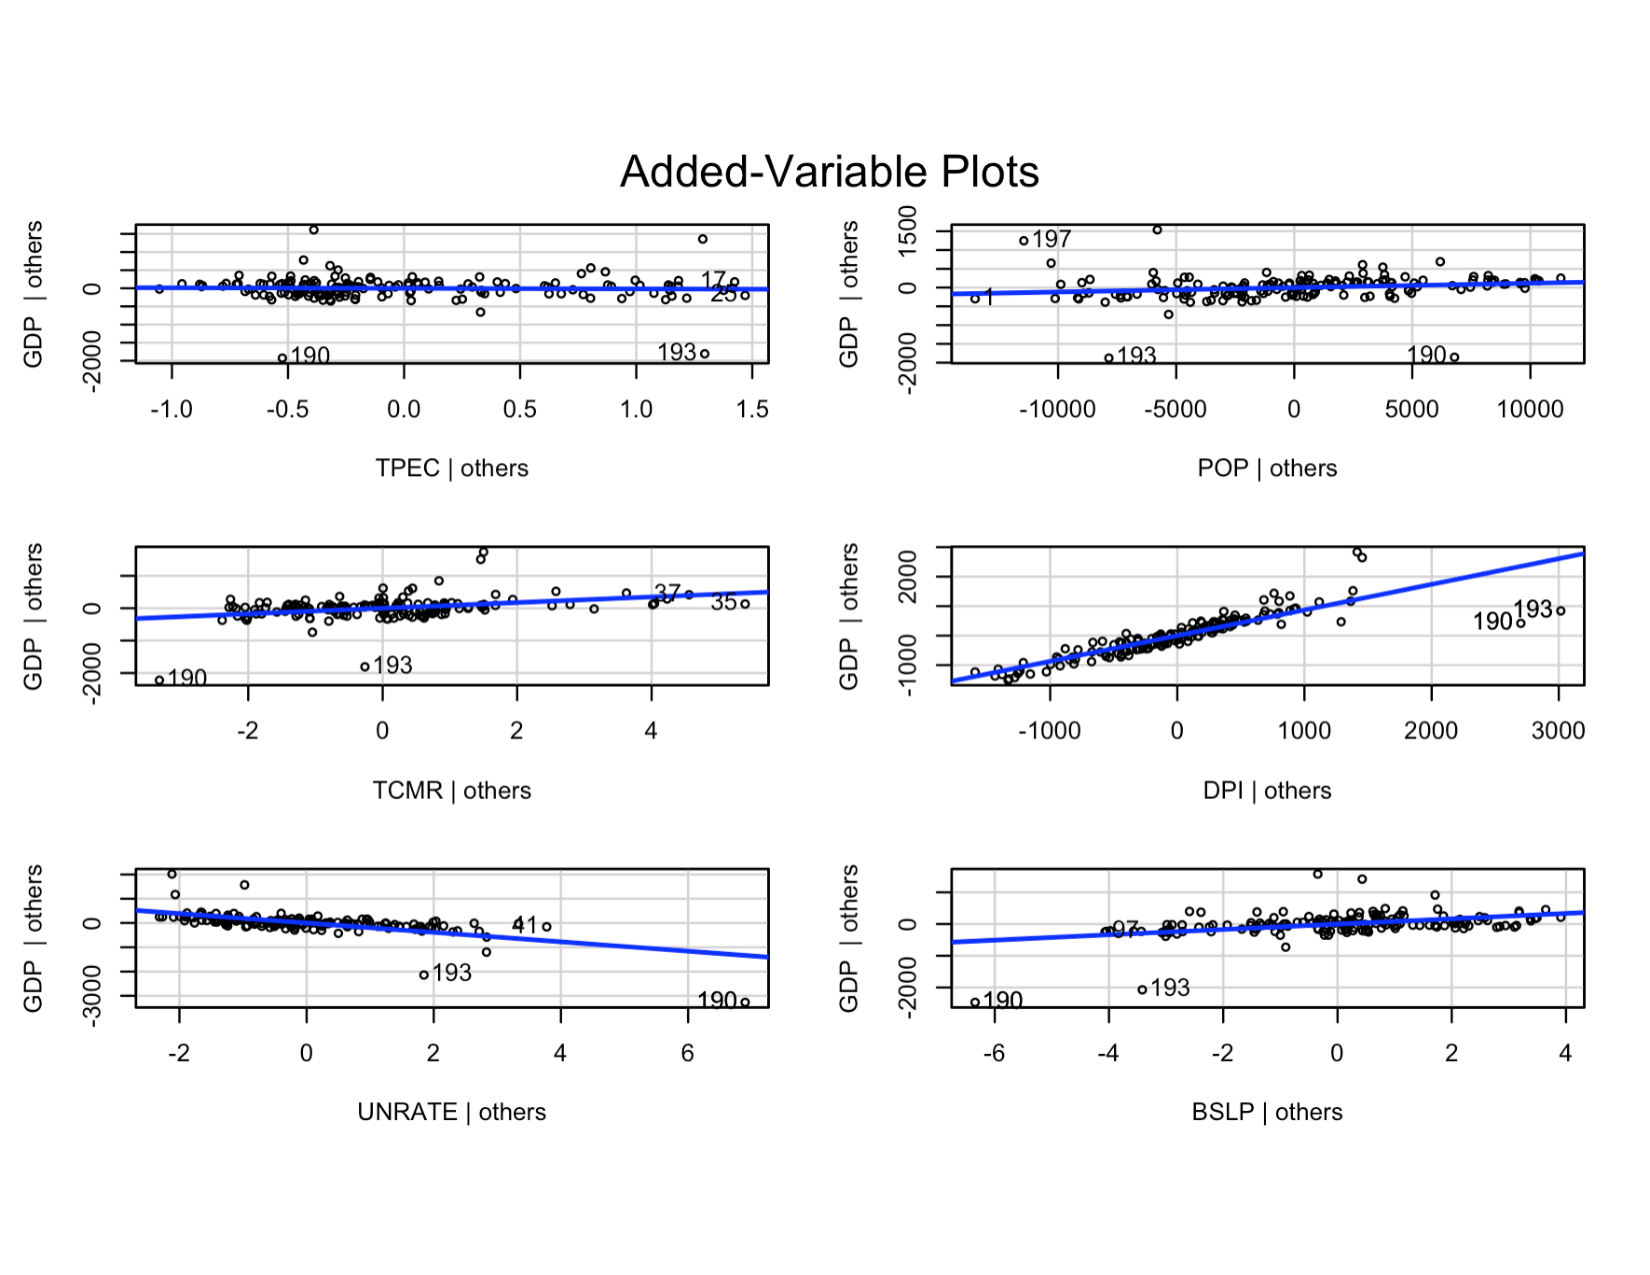
\includegraphics[width=\textwidth]{AVP1}
\end{figure}


\paragraph{Discussion}


\paragraph{Appendix}


\bibliography{refrences}
\bibliographystyle{chicago}

\end{document}